
A partir da construção de uma base de conhecimento,  motor de inferência e de um especialista, o sistema é capaz de realizar soluções esperadas por seres humanos. Estimula-se uma série de regras nas quais determinam alguns fatores importantes para que o sistema possa tomar uma decisão sobre o determinado assunto, e então é trazido o possível resultado encontrado pelo sistema com base nas respostas do usuário.

Da mesma forma que ocorre com as pessoas, para que uma pessoa seja especialista em uma área específica, ela precisa estudar, treinar e se aprofundar  neste assunto para se tornar especialista naquilo.
O sistema especialista geralmente é alimentado por uma pessoa especialista em determinada área e utiliza os requisitos citados acima para se tornar um especialista na tomada de decisão e descobrir a resposta correta que o usuário precisa, sem ter de pedir uma resposta exata daquilo que ele deve encontrar. \cite{Jones}

É uma área da Inteligência Artificial muito usada na área da saúde, principalmente por médicos, para facilitar na descoberta por doenças e ter auxílio para dar a pescrição médica ao paciente. Conforme cita \citeonline{Renato}, "os sistemas especialistas estão sendo utilizados de forma rotineira em muitos setores da atividade humana".
Empresas que trabalham com transações de cartão precisam ter uma decisão rápida de aprovação ou não, e por este motivo também é utilizado este conceito.

\begin{figure}[H]
    \centering
    \caption{Processo de um sistema especialista}
    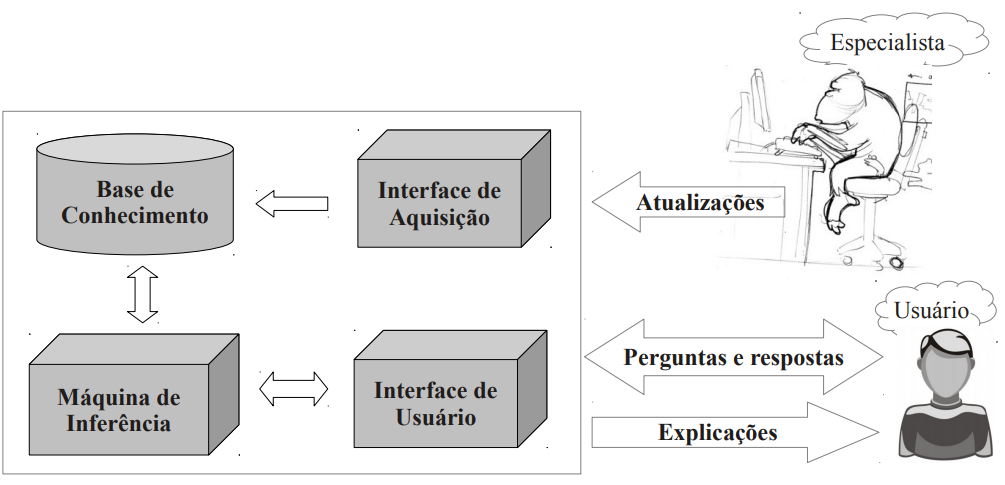
\includegraphics[width=0.8\textwidth]{figura1.PNG}
    \label{processosistema}
    \fonte{\cite{jacsonsilva}}
\end{figure}

A base de conhecimento é o local onde ficam salvas as regras e os fatos. Onde pode ser estruturado e codificado de qualquer maneira para que atinja os resultados desejados.

O motor de inferência ou mecanismo de inferência como também pode ser chamado, pode ser melhor explicado por
\cite{antoniopereira} "É o processo ou interpretação do conhecimento sendo considerado, o coração do mesmo. A principal função é combinar o conhecimento abstrato contido na base regras com o conhecimento concreto armazenado na base de fatos, inferindo conclusão e gerando novos fatos".

Interface do usuário, também possui um papel importante que é realizar a comunição com o usuário através de perguntas e respostas.

O mecanismo de base do interpretador utiliza o encadeamento para frente (\textit{forward}) e encadeamento para trás (\textit{backward}). \citeonline{jacsonsilva} descreve a diferença entre os encadeamentos.

\begin{itemize}
    \item Encadeamento para frente, controle progressivo ou \textit{forward-chaining}: as regras são no sentido condições-conclusões. Dadas as regras, tenta-se usá-las como evidências para construir novos conhecimentos.
    \item Encadeamento para trás: controle regressivo ou \textit{backward-chaining} raciocínio guiado por um
objetivo. Usa-se das regras da base de conhecimento para responder as perguntas. Regras no sentido conclusões-condições.
\end{itemize}

\begin{figure}[H]
    \centering
    \caption{Encadeamento forward e backward}
    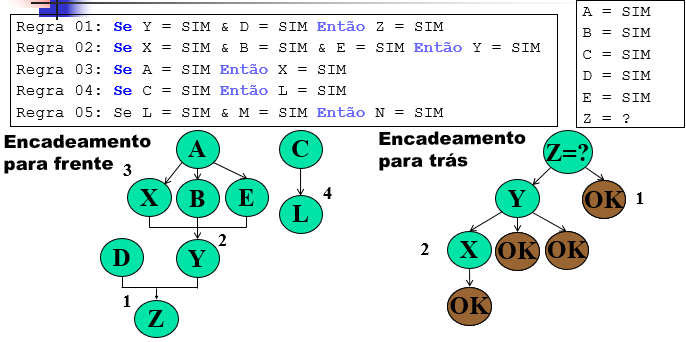
\includegraphics[width=0.8\textwidth]{encadeamento.PNG}
    \label{encadeamento}
    \fonte{\cite{anne}}
\end{figure}


\subsection{Expert Sinta}
\label{expertsinta}

O expert sinta foi desenvolvido pelo  Laboratório de Inteligência Artificial da Universidade Federal do Ceará e é muito conhecido quando se trata de sistemas especialistas. É um software \textit{open source} que foi desenvolvido à algum tempo, mas que por ser muito fácil de utilizar se torna uma ferramenta de grande valor. \cite{Jones}

O software possui interfaces para a manipulação de regras, especificação dos objetivos e criação das variáveis. Possui uma tela para que seja possível observar por quais regras o sistema especialista está passando e deixando gravado as respostas que o usuário informa.

Sistema especialista é baseado em regras que são basicamente conjunto de palavras e fatos com condições e conclusões. É atribuído variáveis para a base de conhecimento e também é estipulado um ou mais objetivos, sendo assim, o processo é iniciado fazendo a pesquisa sobre as regras que possuem o objetivo informado e vai fazendo um encadeamento diante das outras regras até que o seu objetivo realmente seja atingido e então retorna a resposta ao usuário.

Abaixo estão algumas imagens que representam as telas do software, juntamente com exemplos desenvolvidos no trabalho.

% \begin{figure}[H]
%     \centering
%     \caption{Criação de Regras}
%     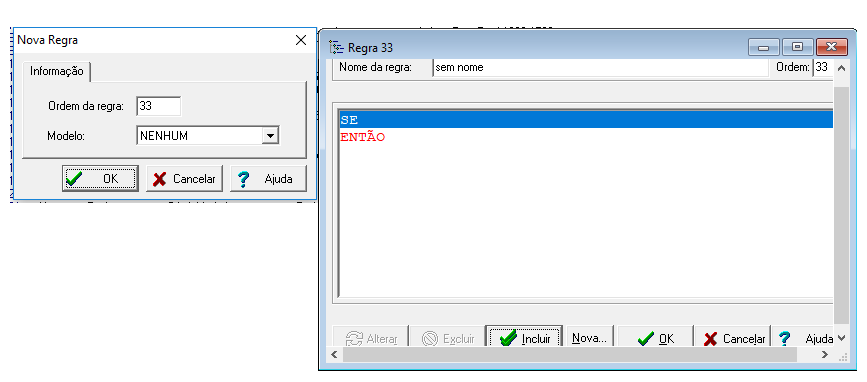
\includegraphics[width=0.8\textwidth]{regra1.PNG}
%     \label{regras1}
%     \fonte{Autor}
% \end{figure}

% \begin{figure}[H]
%     \centering
%     \caption{Consulta de regras criadas}
%     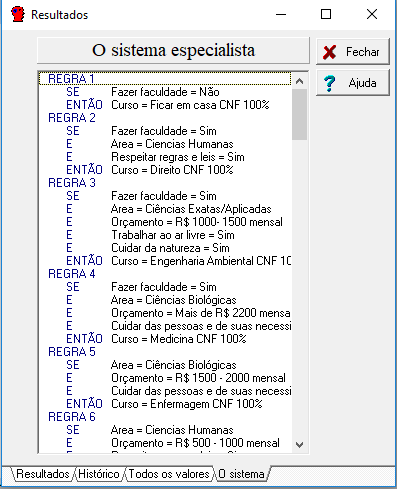
\includegraphics[width=0.8\textwidth]{regras2.PNG}
%     \label{regras2}
%     \fonte{Autor}
% \end{figure}

\begin{figure}[H]
    \centering
    \caption{Regra existente no sistema desenvolvido}
    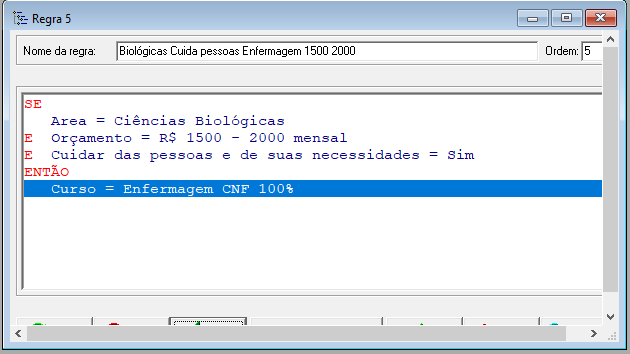
\includegraphics[width=0.8\textwidth]{regras.PNG}
    \label{regras}
    \fonte{Autor}
\end{figure}
A figura \ref{regras} mostra uma das regras que foi criada. O padrão normalmente é este, dá-se três condições e a conclusão é o que está dentro do ENTÃO. Neste caso, se o usuário escolher uma área como sendo Ciências Biológicas, selecionando um valor médio de gasto entre 1500 e 2000 reais mensais, e o perfil dele é de gostar de cuidar das pessoas e de suas necessidades, então o sistema entenderá que deve recomendar o curso de Enfermagem.
 
 
 \begin{figure}[H]
    \centering
    \caption{Criação de Variáveis}
    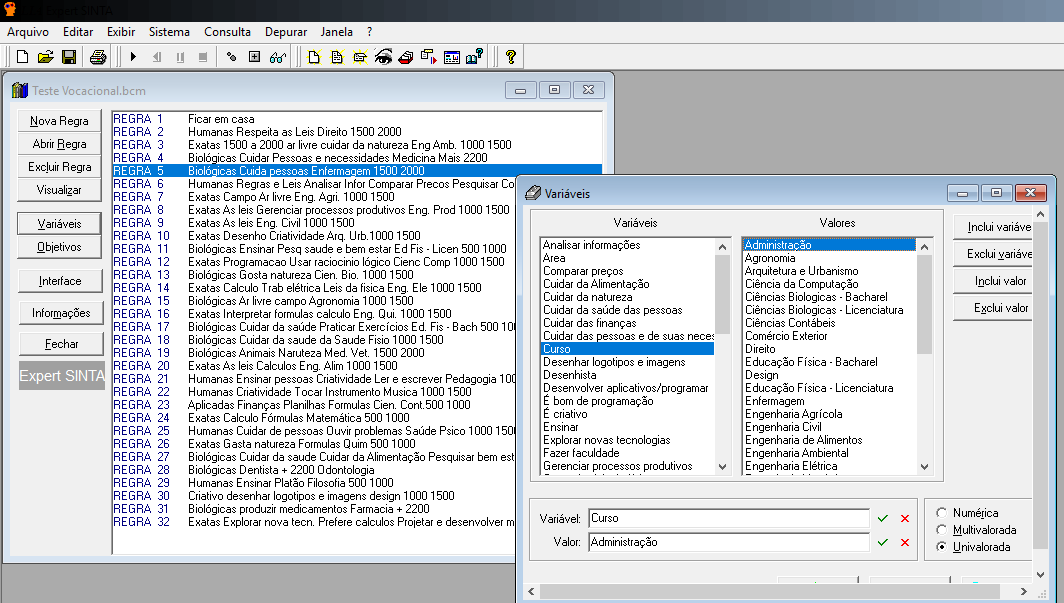
\includegraphics[width=0.8\textwidth]{variaveis.PNG}
    \label{variaveis}
    \fonte{Autor}
\end{figure}
 As variáveis, podem ser criadas para que contenham mais de um único valor, ou seja, marcando a opção multivalorada é possível adicionar mais de um valor à ela. Foi utilizado a variável curso como um exemplo de variável multivalorada.
 
 
  \begin{figure}[H]
    \centering
    \caption{Especificação dos Objetivos}
    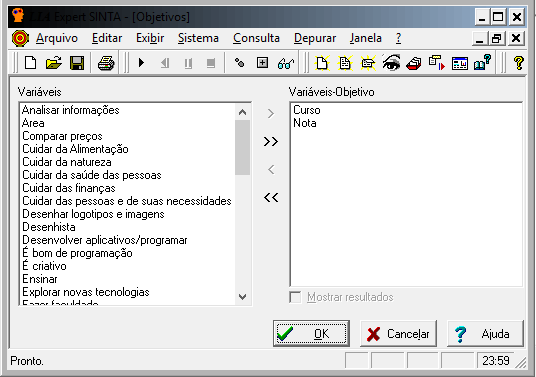
\includegraphics[width=0.8\textwidth]{objetivos.PNG}
    \label{objetivos}
    \fonte{Autor}
\end{figure}

% \begin{figure}[H]
%     \centering
%     \caption{Repostas do usuário}
%     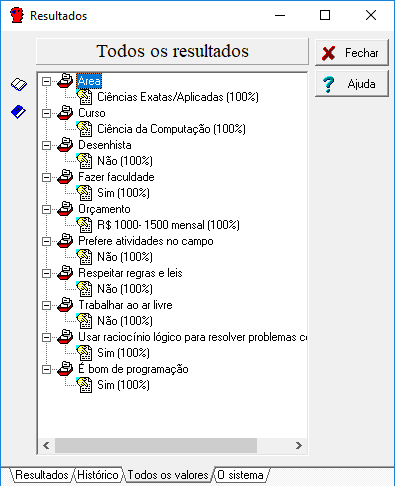
\includegraphics[width=0.5\textwidth]{regras3.PNG}
%     \label{regras3}
% \fonte{Autor}
% \end{figure}

O sistema não irá perguntar diretamente para o usuário sobre a resposta que ele quer, ele irá fazer uma série de outras perguntas, que indiretamente será capaz de descobrir o resultado final, sem que o usuário tenha dito exatamente a sua resposta desejada.


\section{Metodologia}
\label{metodologia}

Utilizou-se a ferramenta Expert Sinta que se encontra no {site}\footnotemark \footnotetext{http://www.lia.ufc.br/~bezerra/exsinta/} para a  realização do trabalho. Levando em conta a facilidade de ser utilizada. Tem por objetivo criar variáveis,  regras com conectivos lógicos e tabelas verdades, assim completando um sistema baseado em conhecimento e fazendo o uso da lógica computacional.

Foi realizado pesquisas sobre as diversas áreas de conhecimento e suas característica para criar as regras, foi recebido auxílio do professor e seu conhecimento sobre o assunto específico da inteligência artificial.



\section{Discussão e Análises dos Resultados}
\label{discussão}
Algumas análises que foram feitas estão baseadas na seguinte regra: para uma pessoa que possui interesse em realizar um curso da área de ciências exatas e gosta de programar, gosta de resolver problemas utilizando raciocínio lógico e pretende gastar um valor médio de 1000,00 a 1500,00, o sistema especialista faz a análise das regras e toma a melhor decisão que é mostrar para o usuário que ele deve realizar o curso de Ciência da Computação. 



